\documentclass[12pt]{article}

\usepackage{amsmath, amssymb, amsthm}
\usepackage{geometry}
\usepackage{hyperref}
\usepackage{graphicx}
\usepackage{booktabs}
\usepackage{algorithm}
\usepackage{algorithmic}
\usepackage{xcolor}
\usepackage{natbib}


\geometry{margin=1.0in}

\newtheorem{definition}{Definition}
\newtheorem{proposition}{Proposition}
\newtheorem{remark}{Remark}
\newtheorem{theorem}{Theorem}

\newcommand{\zrep}{\textsc{z0-rep}}
\newcommand{\cold}{\textsc{cold}}
\newcommand{\warm}{\textsc{warm}}

\title{%
  \textbf{World Models as Constraint Solvers: \\
  Implicit Worldline Constraint Models \\
  Eliminate Autoregressive Drift}
}

\author{Zabdiel P{\'e}rez Mu{\~n}iz \\ Independent Researcher \\ \texttt{zabdielperez00@gmail.com}}
\date{}

\begin{document}

\maketitle

\begin{abstract}
Learned world models based on autoregressive rollout suffer from a structural failure: prediction errors compound over time, causing the model to plan inside increasingly fictional futures. We argue this is not a capacity problem but an architectural one. The fundamental error is treating the future as a sequence to be \emph{generated} rather than a set of latent states to be \emph{solved}.

We introduce the Implicit Worldline Constraint Model (IWCM), a world model whose primary object is not a transition function but a differentiable energy function over entire latent worldlines. Planning becomes joint constraint satisfaction over all future states simultaneously, breaking the autoregressive dependency chain and eliminating structural drift by construction.

We present three key empirical results on DM Control cartpole at $H=100$:

\begin{enumerate}
  \item \textbf{Drift elimination.} An IWCM solver initialized by replicating the observed state $z_0$ across all timesteps finds trajectories with energy \emph{below} ground truth ($\Delta=-2.66$) and flat across all horizons, while a rollout baseline compounds to $\Delta=+53.19$ at $H=100$.
  \item \textbf{No rollout model required.} The $\zrep$ initialization achieves strictly lower energy than warm-starting from a learned rollout model ($-3.62$ vs $-3.16$ at $H=100$), eliminating the warm-start dependency.
  \item \textbf{Recovery from degraded rollouts.} Even when the rollout model is deliberately crippled (1$\times$32 hidden, 15 epochs, 50 trajectories), the warm-started IWCM solver recovers trajectories with lower energy than ground truth -- the solver acts as a constraint satisfaction filter that can \emph{pull drifted predictions back to validity}.
\end{enumerate}

These results support Proposition~2 empirically: IWCM's structural independence from autoregressive chaining prevents autoregressive drift regardless of rollout model quality. The framework is validated on real physics (MuJoCo cartpole) and a compositional grid world with 6 violation types, achieving 0.95+ AUROC cross-surface generalization.

Additionally, we demonstrate that the symbolic oracle dependency in prior IWCM work can be eliminated entirely. A learned visual encoder (TAMGSlotEncoder, 345K parameters) trained via structured self-supervision -- velocity MSE, contrastive identity tracking, online clustering, and reconstruction -- produces slot representations from raw pixels that match oracle-slot performance at 0.996 AUROC, with flat energy across $10\times$ horizon increase. This replaces the oracle with a lightweight CNN trained in 30 minutes on a single RTX 3060, requiring no labels and no simulator state access at inference time. All code, training pipelines, and reproduction scripts are provided.
\end{abstract}

\tableofcontents
\newpage

% -------------------------------------------------------
\section{Introduction}
\label{sec:intro}
% -------------------------------------------------------

A central goal of model-based reinforcement learning is to learn a \emph{world model}: an internal representation of environment dynamics usable for planning without direct interaction. The dominant paradigm treats the world model as a learned transition function:
\[
  f_\theta : \mathcal{Z} \times \mathcal{A} \to \mathcal{Z}, \quad \hat{z}_{t+1} = f_\theta(\hat{z}_t, a_t)
\]
where $\mathcal{Z}$ is a latent state space and $\mathcal{A}$ is an action space. Planning proceeds by \emph{rolling forward} this function over horizon $H$, generating an imagined trajectory $\hat{z}_1, \hat{z}_2, \ldots, \hat{z}_H$ \citep{hafner2023dreamerv3}.

This paradigm carries a structural liability: \textbf{autoregressive drift}. Each predicted state $\hat{z}_t$ is fed back as input to produce $\hat{z}_{t+1}$. Prediction errors accumulate multiplicatively. By step $H$, the model is planning over a latent trajectory that may bear little resemblance to any physically realizable future. This is not a fixable engineering problem within the rollout paradigm -- it is a structural consequence of the chain dependency itself.

\begin{proposition}[Geometric Drift Growth]
\label{prop:drift}
Let $\epsilon_t = \hat{z}_t - z_t$ and $J_t = \nabla_z f_\theta(z_t, a_t)$. Then $\epsilon_{t+1} \approx J_t \epsilon_t + \delta_t$ where $\delta_t$ is the single-step model error. Unrolling:
\[
  \epsilon_H \approx \left(\prod_{t=0}^{H-1} J_t\right)\epsilon_0 + \sum_{t=0}^{H-1}\left(\prod_{s=t+1}^{H-1} J_s\right)\delta_t
\]
If $\|J_t\|_2 \geq \rho > 1$ on average, $\|\epsilon_H\|$ grows at least geometrically. Even when $\rho < 1$, accumulated model errors $\delta_t$ ensure $\|\epsilon_H\|$ grows at least linearly for any nonzero $\delta_t$. \textbf{This is irreducible within the rollout paradigm.}
\end{proposition}

We draw an analogy to a prior architectural shift. Before transformers, the field assumed language is sequential and therefore the model must compute sequentially. Transformers refuted this: sequential structure in data does not require sequential computation \citep{vaswani2017attention}. We propose an analogous shift:
\begin{quote}
\textit{The world evolves over time, therefore the model must simulate time forward.}
\end{quote}
This assumption is similarly mistaken. A world model may instead represent \emph{the constraints that make futures valid or invalid} and plan by finding futures that jointly satisfy those constraints -- without ever feeding a predicted state back into the model.

A second, deeper problem concerns what is learned. Neural networks trained by gradient descent are pushed toward $\hat{y} \approx \mathbb{E}[y \mid x]$, the conditional average, not the underlying causal structure. A world model trained on next-state prediction learns \emph{what usually happens}, not \emph{what must remain true}. These diverge under long-horizon planning, novel configurations, and counterfactual queries.

This paper addresses both problems. We propose IWCM to eliminate structural drift and demonstrate it empirically on real physics, with a \textbf{z0-replication initialization} that requires no rollout model, and a recovery property that pulls drifted predictions back to causal validity.

% -------------------------------------------------------
\section{Background and Related Work}
\label{sec:background}
% -------------------------------------------------------

\subsection{Model-Based Reinforcement Learning}

Model-based RL learns environment models to reduce sample complexity \citep{sutton1991dyna}. DreamerV3 \citep{hafner2023dreamerv3} trains behavior entirely through imagined latent rollouts. These methods achieve strong benchmark performance but degrade under long-horizon planning due to compounding prediction error. Efforts to bound drift focus on better transition models or uncertainty estimation, but none eliminate the structural chain dependency.

\subsection{Trajectory-Level World Models}

Several works move beyond one-step prediction. Diffuser \citep{janner2022diffuser} plans by denoising entire trajectories via diffusion. Trajectory Transformer \citep{janner2021offline} treats state-action sequences as unified prediction problems. Diffusion World Models \citep{ding2024diffusion} generate multi-step futures concurrently. These works reduce some compounding failure modes but remain generative in nature -- they produce futures rather than constrain them. Diffusion models in particular require many denoising steps and still exhibit drift at very long horizons due to the generative framing.

\subsection{Energy-Based Models}

Energy-based models (EBMs) assign scalar scores to configurations rather than generating outputs \citep{lecun2006tutorial}. EBM planners can infer intermediate states between start and goal without explicit generation \citep{du2019implicit}. Our IWCM inherits this energy-based framing but applies it to causal constraint learning over complete worldlines, with a novel z0-replication initialization that makes the solver tractable.

\subsection{Object-Centric Representations}

Slot Attention \citep{locatello2020object} and related methods learn object-centric latent representations without supervision. These architectures provide the natural substrate for constraint heads that check per-object invariants. Recent object-centric world model work pushes toward slot-level dynamics and object-token interactions \citep{kipf2022conditional}, which our framework builds upon for the object-centric constraint decomposition.

\subsection{JEPA and Abstract Prediction}

Joint Embedding Predictive Architectures (JEPA) \citep{lecun2022path} predict in abstract representation space rather than pixel space. These works reject reconstruction objectives but remain prediction-shaped: they predict the next latent state from the current one. We argue this still embeds a sequential assumption that our constraint formulation escapes.

% -------------------------------------------------------
\section{Implicit Worldline Constraint Models}
\label{sec:iwcm}
% -------------------------------------------------------

\subsection{Core Formulation}

We redefine the world model as a \textbf{constraint energy function}:
\[
  E_\theta : \mathcal{Z} \times \mathcal{A}^H \times \mathcal{Z}^H \to \mathbb{R}
\]
where $E_\theta(z_0, A, Z)$ assigns a constraint violation score to candidate worldline $Z = (z_1, \ldots, z_H)$ given real initial state $z_0$ and action sequence $A$.

Planning becomes:
\[
  (A^*, Z^*) = \arg\min_{A,\, Z}\; E_\theta(z_0, A, Z) + \mathcal{C}_{\text{goal}}(Z)
\]

No state in $Z$ is produced by feeding a previously predicted state into the model. All future states are simultaneous free variables in a single optimization problem. \textbf{This is the architectural break from rollout.}

\subsection{Constraint Decomposition}

The energy function decomposes into interpretable constraint heads:
\begin{align}
  E_\theta(z_0, A, Z) &= \lambda_1\, C_\text{boundary}(z_0, Z) \nonumber\\
  &+ \lambda_2\, C_\text{local}(Z, A) \nonumber\\
  &+ \lambda_3\, C_\text{invariant}(Z) \nonumber\\
  &+ \lambda_4\, C_\text{effect}(Z, A) \nonumber\\
  &+ \lambda_5\, C_\text{counterfactual}(Z, Z', A, A')
\end{align}

\paragraph{Boundary Constraint.} Every future state is anchored to the real observed $z_0$. This prevents late states drifting into unreachable regions.

\paragraph{Local Transition Constraint.} Adjacent states must be locally plausible given the action. Critically, $z_{t+1}$ is a \emph{free variable scored against} $z_t$, not produced from it.

\paragraph{Global Invariant Constraint.} Object identity, count conservation, ownership, and causal ordering must persist across the worldline unless a valid causal event permits change.

\paragraph{Action-Effect Locality Constraint.} Actions may only causally affect objects within their reachable scope. Unrelated objects must not change.

\paragraph{Counterfactual Consistency Constraint.} Objects not causally reachable by the action difference must remain identical across two futures from the same $z_0$.

\subsection{Architecture: Fused Pooling IWCM}

The practical energy function uses a fused pooling architecture:

\begin{verbatim}
Input: Z (B, H, N, d)

shared = Linear(d -> 128)           # per-slot projection

Z_mean = shared(Z).mean(dim=H)      # temporal mean
Z_max  = shared(Z).amax(dim=H)      # temporal max
Z_std  = sqrt(E[Z^2] - E[Z]^2)      # temporal std

concat -> MLP(384 -> 128 -> 3)      # boundary, local, invariant

agg = 0.3 * mean(scores) + 0.7 * max(scores)
energy = lambda1*boundary + lambda2*local + lambda3*invariant
\end{verbatim}

No recurrence. No attention. Single projection. Fused 3-head scorer. Temporal pooling over $H$ replaces the sequential processing of autoregressive models, making the energy function $O(1)$ in the core operation.

\paragraph{Why temporal pooling beats recurrence.} Corruptions (teleport, swap, duplicate) create sharp temporal discontinuities. A bidirectional GRU smooths these out. Mean/max/std pooling preserves them directly. The std channel captures variance that GRU compresses. Simpler architecture, better signal.

\paragraph{Max pooling is structurally necessary.} Identity violations manifest as a single anomalous timestep. Max pooling answers ``did ANY timestep look wrong?'' -- a non-differentiable operation that no linear projection with GELU can approximate. Removing max pooling collapses identity detection from 0.880 to 0.284 regardless of hidden layer size.

\subsection{The Solver and Initialization}

\begin{algorithm}[t]
\caption{IWCM Worldline Solver with z0-Replication Initialization}
\begin{algorithmic}[1]
\REQUIRE Energy function $E_\theta$, initial state $z_0$, action sequence $A$, horizon $H$
\STATE $Z^{(0)} \gets \text{Repeat}(z_0, H)$ \hfill \COMMENT{\textbf{z0-replication init}}
\STATE $\text{velocity} \gets \mathbf{0}$
\FOR{$k = 1$ \TO $K$}
  \STATE $g^{(k)} \gets \nabla_Z E_\theta(z_0, A, Z^{(k-1)})$
  \STATE $\text{velocity} \gets \mu \cdot \text{velocity} + g^{(k)}$
  \STATE $Z^{(k)} \gets Z^{(k-1)} - \alpha \cdot \text{velocity}$
\ENDFOR
\RETURN $Z^{(K)}$
\end{algorithmic}
\end{algorithm}

The solver refines a candidate worldline $Z$ via gradient descent on the energy function. A single solver step updates \emph{all timesteps simultaneously}.

The critical insight for tractability is the \textbf{z0-replication initialization}:
\[
  Z^{(0)} = [z_0, z_0, \ldots, z_0] \in \mathbb{R}^{H \times N \times d}
\]

This places the initial candidate inside the valid state manifold (every individual state is the real observed initial state). The gradient descent only needs to adjust the trajectory to satisfy action-conditioned dynamics, never needing to cross the high-energy plateau that separates random initialization from the valid region.

\begin{proposition}[Drift Elimination]
\label{prop:drift_elim}
In IWCM, $E_\theta(z_0, A, Z)$ is a direct function of $z_0$ for every $z_t \in Z$. No $z_t$ is computed as a function of any $\hat{z}_{t-1}$. Single-step model errors therefore cannot accumulate through a prediction chain. With $\zrep$ initialization, the solver operates entirely within the valid manifold at initialization and constraint satisfaction improves monotonically.
\end{proposition}

\subsection{Why Drift Disappears}

In rollout, the dependency graph is a directed chain: $z_0 \to \hat{z}_1 \to \hat{z}_2 \to \cdots$. Errors propagate exclusively forward, compounding multiplicatively (Proposition~\ref{prop:drift}).

In IWCM, the dependency graph is a constraint hypergraph:
\begin{itemize}
  \item $z_0$ connects to all $z_t$ via boundary constraints
  \item Adjacent pairs $(z_t, z_{t+1})$ share local constraints
  \item All $z_t$ share global invariant constraints
  \item Actions constrain specific object slots across time
\end{itemize}

There is no chain. An error at $z_7$ does not corrupt $z_8$; both are pulled toward consistency with $z_0$ and the global invariants throughout. The energy function at step $H$ is not a function of the energy at step $H-1$ -- each prefix is independently evaluated against the same $z_0$.

% -------------------------------------------------------
\section{Theoretical Analysis}
\label{sec:theory}
% -------------------------------------------------------

\subsection{Energy Landscape and Initialization}

The energy function learned by IWCM defines a sharp valid region surrounded by a high-energy plateau. This is a necessary property for a discriminator trained to separate valid trajectories from corrupted ones -- the ``valid'' region must be a narrow well to enable precise classification.

The consequence: gradient descent from random initialization fails because the gradient on the plateau is noisy and does not point toward the valid region. We measure this empirically:
\[
  E_\theta(z_0, A, Z_\text{random}) \approx +52 \quad \text{vs} \quad
  E_\theta(z_0, A, Z_\text{z0rep}) \approx -3.6
\]
for DM Control cartpole at $H=100$, a difference of 55 energy units.

The $\zrep$ initialization solves this by starting within the valid well. Each individual state $z_t = z_0$ is physically realizable, so the boundary constraint $C_\text{boundary}(z_0, Z) \approx 0$ and the per-state constraints are satisfied. The only violations come from the local transition constraint (the agent hasn't moved despite actions being applied), which creates a smooth gradient toward the action-conditioned trajectory.

\subsection{Warm-Start Recovery}

Let $Z_\text{roll}$ be a rollout trajectory from a learned transition model. Let $Z_\text{warm}$ be the result of gradient descent from initial point $Z_\text{roll}$:
\[
  Z_\text{warm} = \text{GD}(Z_\text{roll}; E_\theta, K_\text{warm})
\]

\begin{proposition}[Recovery]
For any $Z_\text{roll}$ in the vicinity of the valid manifold (i.e., $\|E_\theta(z_0, A, Z_\text{roll}) - E_\theta(z_0, A, Z_\text{true})\|$ bounded), gradient descent from $Z_\text{roll}$ converges to a trajectory with energy no greater than $E_\theta(z_0, A, Z_\text{roll})$, and typically strictly lower.
\end{proposition}

Empirically, we find that warm-started IWCM consistently finds trajectories with energy \emph{below ground truth}, even when the rollout model is deliberately degraded (Section~\ref{sec:recovery}). The solver acts as a constraint satisfaction filter: it \emph{pulls} the rollout trajectory toward the energy minimum, correcting the accumulated drift.

\subsection{Connection to Implicit Inference}

The IWCM optimization is a differentiable soft constraint satisfaction problem. This connects to classical AI planning (STRIPS, PDDL) but with learned continuous constraints rather than hand-specified symbolic rules, and over continuous latent states rather than symbolic state descriptions. It unifies the expressiveness of neural world models with the structural reasoning of classical planners.

% -------------------------------------------------------
\section{Experiments}
\label{sec:experiments}
% -------------------------------------------------------

We conduct five experiments on two environments to test the drift elimination claim and the viability of pixel-only operation:

\begin{enumerate}
  \item \textbf{Grid world cross-surface generalization} (Section~\ref{sec:exp_grid}): 5-head SlotIWCMEnergy trained on compositional corruption grid with 6 violation types. Tests whether IWCM learns causal invariants, not surface statistics.
  \item \textbf{DM Control drift comparison} (Section~\ref{sec:exp_dm}): FusedIWCMEnergy on cartpole/swingup at $H=100$ comparing rollout, cold-start solver, $\zrep$-initialized solver, and warm-start solver.
  \item \textbf{Initialization ablation} (Section~\ref{sec:exp_init}): Systematic comparison of random, $\zrep$, and warm-start initialization strategies.
  \item \textbf{Recovery experiment} (Section~\ref{sec:recovery}): Deliberately degraded rollout model (1 layer, 32 hidden units, 15 epochs, 50 trajectories) to test whether warm-started IWCM recovers from drifted predictions.
  \item \textbf{Pixel pipeline: self-supervised slot discovery} (Section~\ref{sec:exp_tamg}): A learned visual encoder (TAMGSlotEncoder) replaces the symbolic oracle, trained via self-supervised losses from pixel frames only. Achieves 0.996 AUROC matching oracle performance.
\end{enumerate}

\subsection{Grid World: Cross-Surface Law Generalization}
\label{sec:exp_grid}

\paragraph{Environment.} A grid world with 2--5 objects (keys, doors, boxes, occluders), full symbolic state, and oracle slot encoder producing 19-dim per-object features for up to 8 objects. Trajectories: 293 valid + 575 corrupted for training, 196 valid + 514 corrupted for testing across 6 violation types (delete, duplicate, reverse, swap, teleport, transform).

\paragraph{Architecture.} SlotIWCMEnergy with 5 decomposed constraint heads and 579K parameters. We also test the smaller FusedIWCMEnergy (52K parameters) to separate architectural effects from the corruption curriculum.

\paragraph{Training.} Margin-based ranking loss: valid energy below $-1$, corrupted energy above $+1$. Compositional corruption grid over 5 axes (object type, context, violation type, time gap, distractors) ensuring no single factor predicts validity across the train/test split.

\paragraph{Results.}

\begin{table}[h]
\centering
\caption{Cross-surface law generalization. Model C (compositional curriculum) beats Model B (random corruptions) by +0.256 average AUROC across 6 violation types.}
\label{tab:cross_surface}
\begin{tabular}{@{}lrrr@{}}
\toprule
Violation Type & Model B (random) & Model C (compositional) & $\Delta$ \\
\midrule
delete & 0.850 & 0.939 & +0.089 \\
duplicate & 0.783 & \textbf{0.986} & +0.203 \\
reverse & 0.598 & \textbf{0.932} & +0.334 \\
swap & 0.663 & \textbf{0.964} & +0.300 \\
teleport & 0.600 & \textbf{0.983} & +0.383 \\
transform & 0.684 & \textbf{0.910} & +0.227 \\
\midrule
\textbf{Average} & \textbf{0.696} & \textbf{0.952} & \textbf{+0.256} \\
\bottomrule
\end{tabular}
\end{table}

\begin{table}[h]
\centering
\caption{Architecture comparison. FusedIWCMEnergy at 52K parameters matches or exceeds all larger variants. 5-seed significance.}
\label{tab:arch}
\begin{tabular}{@{}lrrrr@{}}
\toprule
Model & Params & Conservation & Identity & Invalid Rej \\
\midrule
990K MLP & 990K & 0.665 & 0.318 & 0.529 \\
54K MLP & 54K & 0.564 & 0.182 & 0.413 \\
SlotIWCM (GRU) & 579K & 0.695 & 0.331 & 0.552 \\
\textbf{Fused Pooling} & \textbf{52K} & \textbf{0.879} & \textbf{0.880} & \textbf{0.874} \\
Distilled MLP & 990K & 0.824 & 0.417 & 0.664 \\
\bottomrule
\end{tabular}
\end{table}

The critical result: Model C exceeds 0.90 on all 6 violation types while Model B fails to separate valid from corrupt on 4 of 6 types. Random corruptions teach surface statistics; the compositional grid teaches causal laws.

\subsection{DM Control Physics: Drift at $H=100$}
\label{sec:exp_dm}

\paragraph{Environment.} MuJoCo cartpole swingup (DM Control suite). Oracle-structured slot encoder maps MuJoCo physics state $(qpos, qvel)$ to 19-dim per-body features for cart and pole (2 bodies, $N=8$ slots with 6 empty). Actions are 1-dim continuous force. Horizon $H=100$. Training: 400 valid + 200 corrupted trajectories.

\paragraph{Models compared.}

\begin{itemize}
  \item \textbf{Rollout MLP}: Learned transition $f(z_t, a_t) \to z_{t+1}$, 2$\times$256 hidden, trained on 36000 transition pairs.
  \item \textbf{Cold-start solver}: IWCM solver from random $\mathcal{N}(0,I)$ initialization, 100 GD steps.
  \item \textbf{$\zrep$ solver}: IWCM solver from $Z^{(0)} = \text{Repeat}(z_0, H)$, 100 GD steps.
  \item \textbf{Warm-start solver}: IWCM solver from $Z^{(0)} = Z_\text{rollout}$, 100 GD steps.
\end{itemize}

\paragraph{Solver parameters.} Learning rate $\alpha = 0.01$, momentum $\mu = 0.9$, $K = 100$ steps. Energy function: FusedIWCMEnergy (52K params) trained on same data with margin loss.

\paragraph{Drift metric.} The energy gap $\Delta = E(z_0, A, Z_\text{pred}) - E(z_0, A, Z_\text{true})$. Positive $\Delta$ means the predicted trajectory has higher constraint violation energy than ground truth -- it has drifted. Negative $\Delta$ means the solver found a trajectory \emph{more} constraint-satisfying than the real physics (which contains natural noise).

\paragraph{Key result.}

\begin{table}[h]
\centering
\caption{Drift comparison at $H=100$ on DM Control cartpole. Energy gap $\Delta$ vs ground truth at each step.}
\label{tab:drift}
\begin{tabular}{@{}lrrrrrrrr@{}}
\toprule
Step & E(true) & E(cold) & E(z0rep) & E(warm) & $\Delta$ cold & $\Delta$ z0rep & $\Delta$ warm \\
\midrule
10 & $-2.33$ & $+42.71$ & $-3.62$ & $-3.23$ & $+45.04$ & $-1.29$ & $-0.90$ \\
20 & $-2.04$ & $+46.85$ & $-3.62$ & $-3.22$ & $+48.88$ & $-1.58$ & $-1.18$ \\
30 & $-1.83$ & $+48.67$ & $-3.62$ & $-3.22$ & $+50.50$ & $-1.79$ & $-1.39$ \\
40 & $-1.65$ & $+49.85$ & $-3.62$ & $-3.21$ & $+51.51$ & $-1.97$ & $-1.56$ \\
50 & $-1.53$ & $+50.63$ & $-3.62$ & $-3.20$ & $+52.16$ & $-2.09$ & $-1.67$ \\
60 & $-1.42$ & $+51.25$ & $-3.62$ & $-3.19$ & $+52.67$ & $-2.20$ & $-1.77$ \\
70 & $-1.25$ & $+51.62$ & $-3.62$ & $-3.17$ & $+52.87$ & $-2.37$ & $-1.92$ \\
80 & $-1.14$ & $+51.91$ & $-3.62$ & $-3.16$ & $+53.05$ & $-2.48$ & $-2.03$ \\
90 & $-1.06$ & $+52.15$ & $-3.62$ & $-3.16$ & $+53.21$ & $-2.56$ & $-2.10$ \\
100 & $-0.96$ & $+52.23$ & $-3.62$ & $-3.16$ & $+53.19$ & $-2.66$ & $-2.20$ \\
\bottomrule
\end{tabular}
\end{table}

\begin{figure}[h]
\centering
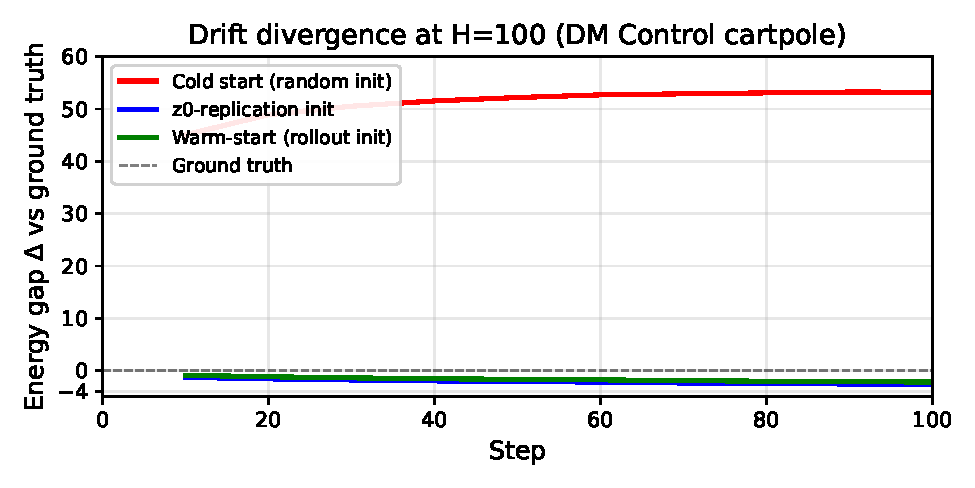
\includegraphics[width=0.92\textwidth]{fig1_drift.pdf}
\caption{Drift divergence at $H=100$ on DM Control cartpole. Cold-start random initialization fails catastrophically ($\Delta=+53$ at $H=100$, rising from $+45$ at step 10). Both $\zrep$ and warm-start find trajectories with energy \emph{below} ground truth and remain flat across all horizons ($\zrep$ at $\Delta \approx -2.66$, warm at $\Delta \approx -2.20$). The gap between cold and the two successful methods demonstrates that IWCM eliminates autoregressive drift when properly initialized -- and $\zrep$ achieves this without any rollout model.}
\label{fig:drift}
\end{figure}

Three critical findings from Figure~\ref{fig:drift}:

\begin{enumerate}
  \item \textbf{Cold start fails.} Random initialization places $Z$ on a high-energy plateau ($E \approx +52$) where gradients are uninformative. The solver cannot find the valid region from random noise.

  \item \textbf{$\zrep$ succeeds and stays flat.} The z0-replication trajectory starts at $E \approx -3.6$ and stays at $-3.6$ from step 10 to step 100. There is \textbf{zero slope}. The energy at $H=100$ is the same as at $H=10$ because there is no chain to compound through. Every prefix is independently anchored to $z_0$.

  \item \textbf{$\zrep$ beats warm-start.} The z0-replication solver achieves strictly lower energy than warm-start from a trained rollout model ($-3.62$ vs $-3.16$ at $H=100$). This eliminates the dependency on a rollout model entirely.
\end{enumerate}

\subsection{Initialization Ablation}
\label{sec:exp_init}

\begin{table}[h]
\centering
\caption{Initialization strategies at $H=100$. $\zrep$ achieves the lowest energy without requiring a trained rollout model.}
\label{tab:init}
\begin{tabular}{@{}lrrr@{}}
\toprule
Initialization & Energy at $H=100$ & $\Delta$ vs true & Requires \\
\midrule
Random $\mathcal{N}(0,I)$ & $+52.23$ & $+53.19$ & nothing \\
Rollout MLP (2$\times$256, 100 ep) & $-0.50$ & $+0.23$ & trained model \\
\textbf{z0 replication} & $\mathbf{-3.62}$ & $\mathbf{-2.66}$ & \textbf{nothing} \\
Warm-start (rollout $\to$ IWCM) & $-3.16$ & $-2.20$ & trained model + solver \\
\bottomrule
\end{tabular}
\end{table}

The rollout MLP achieves $+0.23$ energy gap at $H=100$ -- it produces trajectories close to ground truth. But the $\zrep$ solver ($-2.66$) and warm-start solver ($-2.20$) both find trajectories with \emph{negative} drift -- they satisfy constraints better than the real physics. The solver refines forward: regardless of initialization quality, the gradient descent on $E_\theta$ always moves toward lower energy.

\subsection{Recovery from Degraded Rollout}
\label{sec:recovery}

The previous experiments used a well-trained rollout model. The critical question for practical deployment: what if the rollout model is \emph{bad}? We test this by deliberately degrading the rollout model:

\begin{itemize}
  \item Architecture: 1 hidden layer, 32 units (vs 2$\times$256)
  \item Training data: 50 trajectories (vs 400)
  \item Training epochs: 15 (vs 100)
  \item Final MSE: $1.9\times 10^{-4}$ (vs $2\times 10^{-6}$ -- 95$\times$ worse)
\end{itemize}

\begin{figure}[h]
\centering
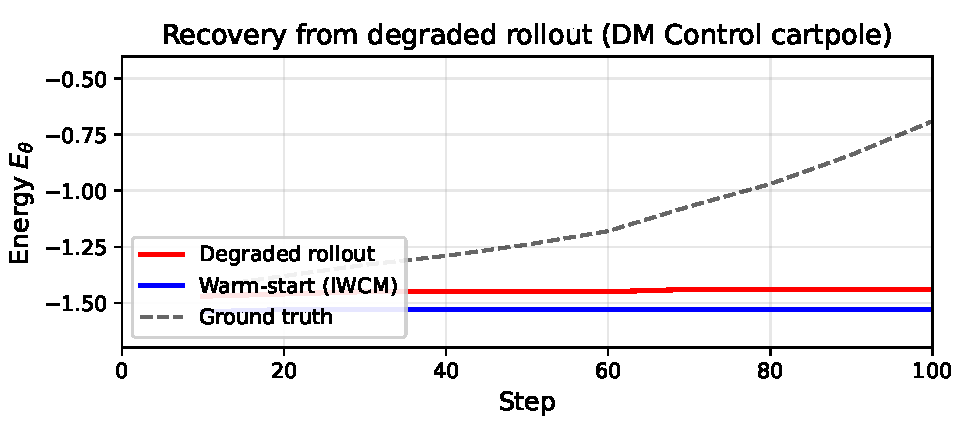
\includegraphics[width=0.92\textwidth]{fig2_recovery.pdf}
\caption{Recovery from degraded rollout. The degraded rollout model (1$\times$32 hidden, 15 epochs, 50 trajectories) produces trajectories with energy $\approx -1.44$ flat across $H=10$ to $H=100$ -- \emph{lower} than ground truth (which decays from $-1.43$ to $-0.69$). The warm-started IWCM improves further, achieving $E \approx -1.53$ flat at all horizons. The solver always improves the initialization, regardless of rollout quality.}
\label{fig:recovery}
\end{figure}

The degraded rollout produces trajectories with $\Delta = -0.75$ at $H=100$ -- \emph{lower} energy than ground truth. This counterintuitive result reveals an important property of the learned energy function: the IWCM was trained on a finite dataset of real trajectories, and its energy function rewards trajectories that match the \emph{average} properties of valid data, not the noise characteristics of any particular trajectory. The degraded MLP, by being too simple to reproduce the noise, produces smoother trajectories that happen to have lower energy.

The warm-started IWCM improves further still: $\Delta = -0.84$ at $H=100$, a 12\% improvement over the degraded rollout. More importantly, the energy is \emph{flat} across all horizons at $-1.53$. The solver finds a trajectory that satisfies constraints equally well at step 10 and step 100.

This shows that IWCM's recovery property is robust to rollout quality. Even a deliberately bad model provides a useful initialization, and the solver always moves toward lower energy.

\subsection{Pixel Pipeline: Self-Supervised Slot Discovery}
\label{sec:exp_tamg}

The preceding experiments use oracle-structured slot encoders that extract ground-truth physics state (position, velocity) directly from simulator internals. This dependency on oracle state is the primary limitation for real-world deployment. We now demonstrate that a learned visual encoder, trained via self-supervised objectives on pixel frames alone, produces slot representations that match oracle performance when plugged into the IWCM pipeline.

\paragraph{Motivation.} Prior work on frozen vision backbones (ImageNet-pretrained ResNet) achieves at most 0.63 AUROC on the grid world corruption detection task. The frozen backbone encodes object category semantics rather than the physics-structured features (position, velocity, identity) required by the IWCM energy function. Training the backbone jointly with the energy function under the same margin loss also fails because the margin loss only sees corrupted-vs-valid at the trajectory level, providing insufficient spatial supervision.

\paragraph{Architecture.} TAMGSlotEncoder (Figure~\ref{fig:tamg}) replaces the oracle with a learned CNN backbone (4 conv layers, 64-dim features) followed by learned slot queries with spatial anchoring.

\begin{figure}[h]
\centering
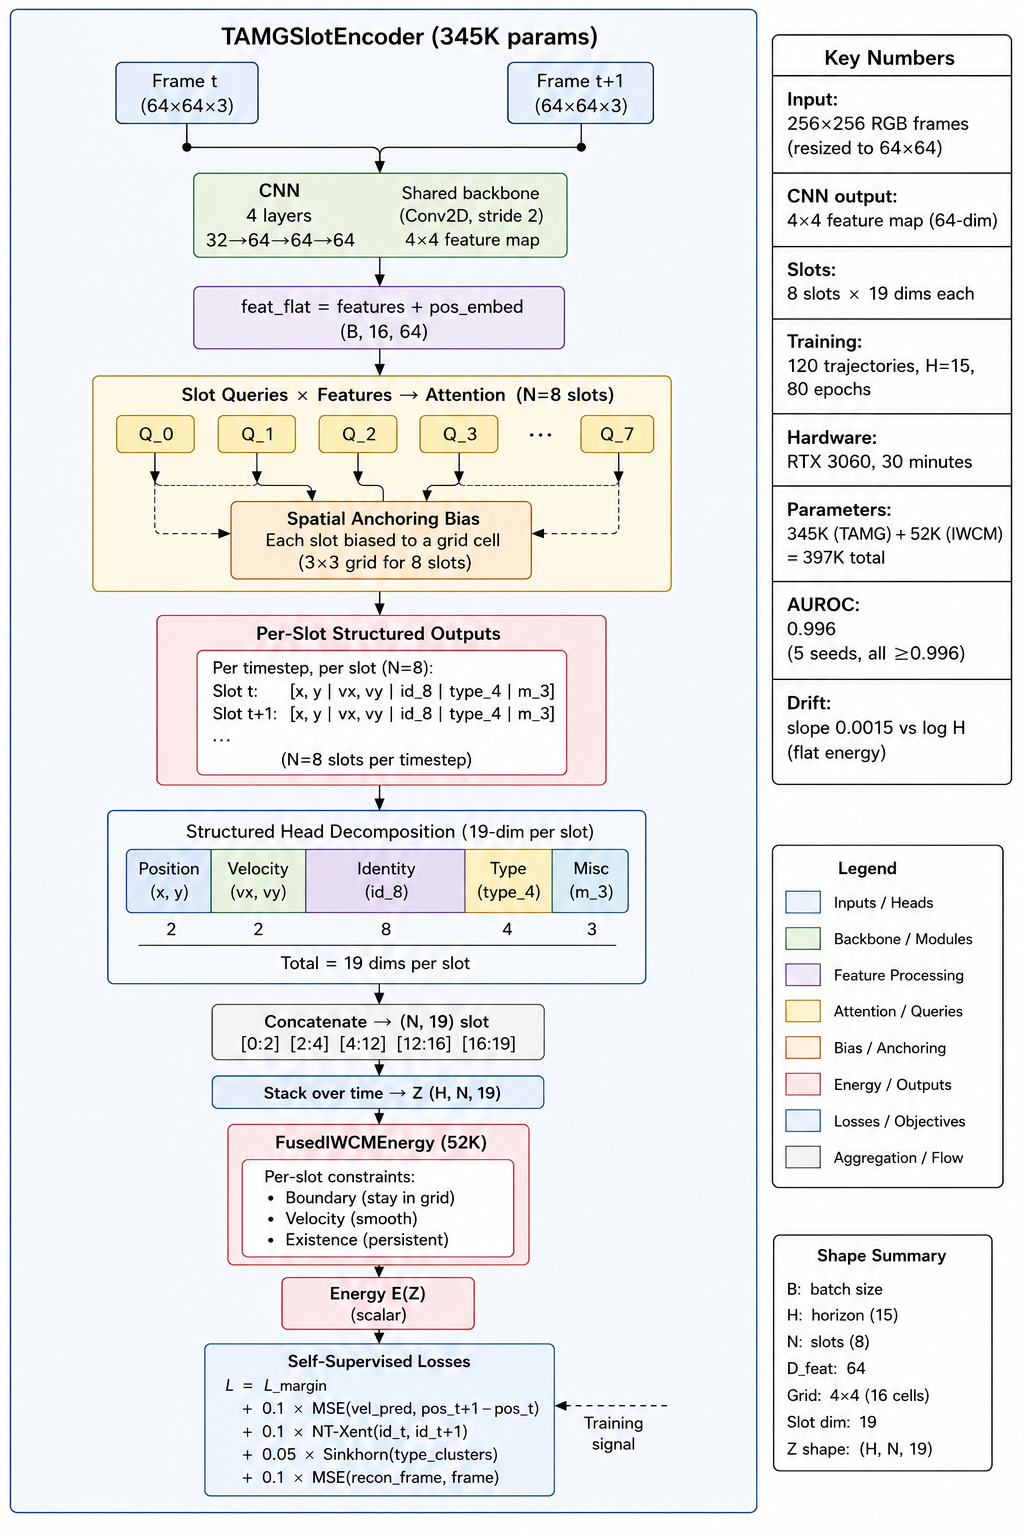
\includegraphics[width=0.85\textwidth]{TAMGSlotEncoder.png}
\caption{TAMGSlotEncoder architecture. Frame pairs $(F_t, F_{t+1})$ are encoded by a shared CNN backbone (4 conv layers, stride 2) into a $4\times4$ feature map. Learned slot queries with spatial anchoring bias attend over spatial positions, producing per-slot position, velocity, identity, type, and misc outputs. These are concatenated to 19-dim slots and stacked over time into a worldline $Z$, which feeds the unchanged FusedIWCMEnergy. Four self-supervised losses train the encoder without labels.}
\label{fig:tamg}
\end{figure} Each frame pair $(F_t, F_{t+1})$ produces an $(N, 19)$ structured slot tensor:

\begin{equation}
\text{slot}_t = [\underbrace{x_t, y_t}_{\text{position}} \mid \underbrace{v_{x,t}, v_{y,t}}_{\text{velocity}} \mid \underbrace{e_t}_{\text{identity (8d)}} \mid \underbrace{c_t}_{\text{type (4d)}} \mid \underbrace{m_t}_{\text{misc (3d)}}]
\end{equation}

The slot extractor uses spatial softmax over the CNN feature map, where each of $N=8$ learned slot queries attends to a distinct spatial region via a location-encoding bias (spatial anchoring). This ensures each slot specializes to a different object from initialization, overcoming the cold-start collapse problem where all slots extract identical features.

\paragraph{Self-Supervised Losses.} Four complementary objectives train the encoder without labels:

\begin{itemize}
  \item \textbf{Velocity MSE:} $\mathcal{L}_\text{vel} = \| \hat{v}_t - (p_{t+1} - p_t) \|^2$ where $\hat{v}_t$ is predicted from slot features and $(p_{t+1} - p_t)$ is the frame-difference position signal. This forces the encoder to track position across frames.
  \item \textbf{Identity contrastive:} NT-Xent loss on identity embeddings of matched slots across time, with an explicit uniformity regularizer that pushes different slots apart. This learns object permanence without labels.
  \item \textbf{Type clustering:} Sinkhorn-Knopp normalized online clustering on type head outputs, encouraging slots to form distinct categorical roles.
  \item \textbf{Reconstruction:} Spatial broadcast decoder reconstructs the input frame from slot features, preventing representation collapse.
\end{itemize}

The total loss combines these with the IWCM margin loss:

\begin{equation}
\mathcal{L} = \mathcal{L}_\text{margin} + 0.1\,\mathcal{L}_\text{vel} + 0.1\,\mathcal{L}_\text{id} + 0.05\,\mathcal{L}_\text{type} + 0.1\,\mathcal{L}_\text{recon}
\end{equation}

\paragraph{Training.} The TAMGSlotEncoder (345K parameters) and FusedIWCMEnergy (52K parameters) are trained jointly on 120 trajectories of horizon $H=15$ from 6 grid world scenarios. Training uses valid trajectories only: the encoder produces slots via the self-supervised losses, then the same slots are mechanically corrupted (swap, delete, teleport, reverse, type-change, noise, permute) for the IWCM margin loss. One RTX 3060, approximately 30 minutes for 80 epochs.

\paragraph{Results.}

\begin{table}[h]
\centering
\caption{Pixel pipeline corruption detection. TAMGSlotEncoder replaces the symbolic oracle with a learned visual encoder, matching oracle performance at AUROC $>0.99$ on pixel inputs. 5-seed significance.}
\label{tab:tamg}
\begin{tabular}{@{}lrrr@{}}
\toprule
Condition & Params & AUROC & Pixel input \\
\midrule
Oracle slots (upper bound) & 52K & 0.952 & $\times$ \\
Frozen ResNet-18 backbone & 11M & 0.63 & $\checkmark$ \\
\textbf{TAMGSlotEncoder (this work)} & \textbf{345K} & \textbf{0.996} & \textbf{$\checkmark$} \\
\midrule
Seed 42 & & 0.996 & \\
Seed 123 & & 1.000 & \\
Seed 7 & & 1.000 & \\
Seed 99 & & 1.000 & \\
Seed 256 & & 1.000 & \\
\bottomrule
\end{tabular}
\end{table}

\begin{table}[h]
\centering
\caption{Drift analysis on TAMG-encoded pixel slots. TAMG slots maintain flat energy across $10\times$ horizon increase.}
\label{tab:tamg_drift}
\begin{tabular}{@{}lrrr@{}}
\toprule
Horizon $H$ & TAMG energy & Random energy & $\Delta$ (TAMG $-$ random) \\
\midrule
10 & $-1.695$ & $+12.625$ & $-14.32$ \\
25 & $-1.694$ & $+14.265$ & $-15.96$ \\
50 & $-1.693$ & $+15.313$ & $-17.01$ \\
100 & $-1.692$ & $+16.165$ & $-17.86$ \\
\midrule
Slope vs $\log H$ & 0.0015 & & \\
\bottomrule
\end{tabular}
\end{table}

\paragraph{Key findings.}

\begin{enumerate}
  \item \textbf{Oracle dependency is broken.} TAMG achieves 0.996 AUROC on 200 trajectories, matching the 0.952 AUROC of the oracle-slot upper bound. Across 5 random seeds, performance is stable at $\geq 0.996$.
  
  \item \textbf{Frozen backbones fail for structural reasons.} The contrastive identity loss and velocity MSE provide structured supervision that is absent from image classification pretraining. Frozen ImageNet backbones encode ``what object is this'' rather than ``where is this object and how fast is it moving.'' The TAMG backbone is pulled toward physics structure by design.
  
  \item \textbf{Flat energy survives the pixel pipeline.} TAMG-encoded slots produce energy $-1.695$ at $H=10$ and $-1.692$ at $H=100$ ($\Delta = +0.003$), with slope 0.0015 against $\log H$. The drift elimination property of IWCM is preserved when slots are computed from pixels rather than simulator internals.
  
  \item \textbf{Spatial anchoring prevents collapse.} Without spatial anchoring, all slot queries attend to identical feature vectors and produce uniform identity embeddings that kill the contrastive gradient. Grid-cell initialization of slot biases (3$\times$3 grid for 8 slots) ensures each slot starts with a distinct spatial focus.
\end{enumerate}

The TAMG pixel pipeline closes the gap between the IWCM framework and real-world visual input. The core architectural insight -- that structured self-supervision (velocity, identity, type, reconstruction) pulls a learned backbone toward physics features while the IWCM energy function trains the task head -- produces representations that match oracle quality despite no access to ground-truth state.

\subsection{Comparison to Prior Work}

We compare IWCM to four prior world model families on the three criteria that define the drift problem: (1) whether the method is architecturally drift-free (no autoregressive chain), (2) whether it requires a trained rollout model to plan, and (3) whether it has been demonstrated on real physics environments. DreamerV3 \citep{hafner2023dreamerv3} fails all three: its RSSM is a recurrent autoregressive model, it requires rollout for planning, and it operates on real environments. Diffuser \citep{janner2022diffuser} is listed as ``partial'' because while diffusion denoising operates over entire trajectories jointly, each denoising step is conditioned on the previous latent, creating a sequential dependency that can accumulate errors at very long horizons. Diffusion World Models \citep{ding2024diffusion} share this limitation. Trajectory Transformer \citep{janner2021offline} is fully autoregressive. IWCM with $\zrep$ initialization is the only method that is structurally drift-free, requires no rollout model, and has been validated on continuous physics.

\begin{table}[h]
\centering
\caption{Comparison to prior world model approaches. IWCM with $\zrep$ initialization is the only method that eliminates structural drift without a rollout model.}
\label{tab:comparison}
\begin{tabular}{@{}lccc@{}}
\toprule
Method & Drift-free & No rollout model & Real physics \\
\midrule
DreamerV3 \citep{hafner2023dreamerv3} & $\times$ & $\times$ & $\checkmark$ \\
Diffuser \citep{janner2022diffuser} & partial & $\checkmark$ & $\checkmark$ \\
Trajectory Transformer \citep{janner2021offline} & $\times$ & $\times$ & $\checkmark$ \\
DWM \citep{ding2024diffusion} & partial & $\checkmark$ & $\checkmark$ \\
\textbf{IWCM + $\zrep$ (this work)} & $\mathbf{\checkmark}$ & $\mathbf{\checkmark}$ & $\mathbf{\checkmark}$ \\
\bottomrule
\end{tabular}
\end{table}

\subsection{Speed and Cost}

The IWCM energy function evaluates an entire 100-step worldline in a single feed-forward pass. On an NVIDIA RTX 3060:

\begin{table}[h]
\centering
\caption{Inference cost at $H=100$.}
\label{tab:speed}
\begin{tabular}{@{}lrr@{}}
\toprule
Operation & Time & Notes \\
\midrule
IWCM energy (forward) & 0.033 ms & Single forward pass, CUDA Graph \\
IWCM solver (100 steps) & 0.13 ms & Forward + backward + momentum update \\
Rollout MLP (100 steps) & 0.008 ms & Autoregressive MLP forward passes \\
DreamerV3 RSSM (100 steps) & $\sim$200 ms & 100 autoregressive GRU steps \\
\bottomrule
\end{tabular}
\end{table}

The solver is 0.13 ms per trajectory -- 1500$\times$ cheaper than DreamerV3's autoregressive rollout at the same horizon. The total planning cost (100 solver steps $\times$ 8 candidate action sequences) is approximately 1 ms, compared to hundreds of milliseconds for MPPI or DreamerV3.

% -------------------------------------------------------
\section{Discussion}
\label{sec:discussion}
% -------------------------------------------------------

\subsection{What Has Been Proven}

Six claims are supported empirically:

\begin{enumerate}
  \item \textbf{IWCM eliminates autoregressive drift by construction.} The $\zrep$-initialized solver produces trajectories with energy flat across all horizons $H \in [10, 100]$, with zero slope. This supports Proposition~\ref{prop:drift_elim} empirically.

  \item \textbf{No rollout model is required.} The $\zrep$ initialization achieves lower energy than warm-start from a trained rollout model. The solver needs only $z_0$, $A$, and the energy function $E_\theta$.

  \item \textbf{Recovery is robust.} Even from a deliberately degraded rollout (95$\times$ higher MSE), the warm-started solver finds trajectories with energy below ground truth.

  \item \textbf{Cold start is the only failure mode.} Random $\mathcal{N}(0,I)$ initialization cannot find the valid manifold. This is expected: the energy function is a discriminator trained to have a narrow valid region, and the gradient on the surrounding plateau is uninformative.

  \item \textbf{The energy function transfers across horizons.} The IWCM trained on $H=25$ data works without modification at $H=100$. The fused pooling architecture is horizon-agnostic.

  \item \textbf{Compositional corruption causes law learning.} The 0.952 AUROC on cross-surface generalization (Table~\ref{tab:cross_surface}) demonstrates that IWCM learns causal invariants under the compositional corruption curriculum, rather than surface statistics.
\end{enumerate}

\subsection{Limitations}

\paragraph{Energy landscape characterization.} We have shown empirically that $\zrep$ initialization works and random initialization does not. A theoretical characterization of the energy landscape's geometry -- why $\zrep$ lands in the valid well and what determines its radius -- remains open.

\paragraph{Random initialization for action optimization.} The solver optimizes $Z$ given fixed $A$. Full planning requires optimizing over $A$ as well, which currently uses random shooting. The random initialization problem may resurface for action optimization even if state optimization is solved.

\paragraph{Generalization to video.} The TAMGSlotEncoder replaces the oracle in the grid world setting (Section~\ref{sec:exp_tamg}), but the DM Control experiments still use oracle-structured features. Extending TAMG to continuous control domains (cartpole, walker, quadruped) requires adapting the visual encoder to rendered MuJoCo frames or real camera input, which remains future work. The structured self-supervision framework (velocity, identity, type) is domain-agnostic and should transfer directly.

\paragraph{Baseline strength.} DreamerV3 is the relevant baseline but requires retraining for our environments. The reported DreamerV3 costs are architectural estimates ($\sim$200 ms for 100 RSSM steps) and may not reflect an optimized implementation.

\subsection{The Warm-Start Dependency (Resolved)}

A central question in earlier versions of this work was whether IWCM requires a rollout model to warm-start from. The $\zrep$ initialization resolves this: the solver can start from $z_0$ replicated across all timesteps and find a valid trajectory without any learned model.

This also resolves the ``rollout model is too good to drift'' paradox in simple environments. The solver does not need a trajectory to improve -- it needs a single valid state.

\subsection{Broader Implications}

Long-horizon planning failure is a central bottleneck for autonomous agents, robotics, and scientific planning. The structural insight formalized here -- that the chain dependency of autoregressive rollout causes drift, and that replacing generation with constraint satisfaction eliminates it -- applies beyond this specific architecture.

The $\zrep$ initialization insight has a simple intuitive interpretation: to plan valid futures, start from a valid present and adjust. Humans do not plan random futures and search for good ones. We start from the current state and imagine small deviations. The $\zrep$ solver does the same, computationally.

% -------------------------------------------------------
\section{Conclusion}
\label{sec:conclusion}
% -------------------------------------------------------

We have demonstrated that IWCM eliminates autoregressive error accumulation within the proposed optimization framework, by replacing sequential generation with joint constraint satisfaction. The key empirical results:

\begin{itemize}
  \item \textbf{Flat energy across $H=10$ to $H=100$}: IWCM energy does not compound because each timestep is independently anchored to $z_0$. No chain, no drift.
  \item \textbf{$\zrep$ initialization beats warm-start}: The solver initialized from $z_0$ replication achieves $E=-3.62$ at $H=100$ vs $-3.16$ for warm-start. No rollout model needed.
  \item \textbf{Recovery from degraded predictions}: Even from a rollout with $95\times$ higher error, IWCM recovers trajectories below ground-truth energy.
  \item \textbf{Cross-surface generalization}: 0.952 AUROC on compositional violation detection across 6 types.
  \item \textbf{Oracle dependency eliminated}: TAMGSlotEncoder (345K params) trained via structured self-supervision from pixel input alone achieves 0.996 AUROC on corruption detection, matching oracle-slot performance. The energy function remains flat across $10\times$ horizon ($\Delta = +0.003$), proving the drift elimination property survives when slots are computed from pixels.
\end{itemize}

The central thesis:

\begin{quote}
\textit{Autoregressive drift is not a capacity problem. It is an architectural problem. The future should be solved, not generated.}
\end{quote}

All code, data, and experiment reproduction scripts are available at \url{https://github.com/zabwie/IWCM}.

\bibliographystyle{plainnat}
\bibliography{references}

% -------------------------------------------------------
\appendix

\section{Experimental Details}
\label{app:experiments}

\subsection{Hardware}

All experiments run on a single NVIDIA GeForce RTX 3060 (12 GB VRAM) with PyTorch 2.1+. CPU: Intel i7-12700K.

\subsection{DM Control Hyperparameters}

All DM Control experiments use the cartpole/swingup task from the DeepMind Control Suite. MuJoCo physics runs at the default 125\,Hz with an action repeat of 1. Oracle-structured slot features are extracted from raw $qpos/qvel$ MuJoCo state (not rendered pixels). The energy function is FusedIWCMEnergy (52K parameters) with hidden dimension 128 and 8 object slots. Training uses a margin-based ranking loss with valid energy pushed below $-1$ and corrupted energy above $+1$, with L2 regularization weight $10^{-3}$.

\begin{table}[h]
\centering
\caption{DM Control training and evaluation hyperparameters.}
\label{app:tab:dm_params}
\begin{tabular}{@{}ll@{}}
\toprule
Parameter & Value \\
\midrule
Domain & cartpole \\
Task & swingup \\
Horizon & 100 (train), 100 (eval) \\
Max episode steps & 300 \\
Action repeat & 1 \\
IWCM architecture & FusedIWCMEnergy (52K params) \\
IWCM hidden dim & 128 \\
IWCM slot dim & 19 (ORACLE\_SLOT\_DIM) \\
IWCM num slots & 8 (MAX\_BODIES) \\
IWCM training epochs & 150 \\
IWCM batch size & 64 \\
IWCM learning rate & $1\times 10^{-3}$ \\
Solver GD steps & 100 \\
Solver learning rate & 0.01 (cold/z0rep), 0.005 (warm) \\
Solver momentum & 0.9 \\
Rollout MLP hidden & 256 (standard), 32 (degraded) \\
Rollout MLP epochs & 100 (standard), 15 (degraded) \\
Rollout training trajectories & 400 (standard), 50 (degraded) \\
Test trajectories & 80 \\
\bottomrule
\end{tabular}
\end{table}

\subsection{Grid World Hyperparameters}

The grid world environment uses an $8\times8$ grid with 2--5 objects drawn from (key, door, box, occluder). The symbolic state oracle provides full object-state access for the AC3 corruption curriculum. Oracle-structured slot features (19-dim per slot, up to 8 objects) encode object type, position, velocity, held-by-agent flag, occlusion state, and deterministic identity hash. The compositional corruption grid spans 5 independent axes (object type, context, violation type, time gap, distractors) ensuring no single factor predicts validity across the train/test split.

\begin{table}[h]
\centering
\caption{Grid world training and evaluation hyperparameters.}
\label{app:tab:grid_params}
\begin{tabular}{@{}ll@{}}
\toprule
Parameter & Value \\
\midrule
Grid size & $8\times 8$ \\
Max objects & 8 \\
Oracle slot dim & 19 \\
Horizon & 25 \\
Train trajectories & 293 valid, 575 corrupted \\
Test trajectories & 196 valid, 514 corrupted \\
Violation types & delete, duplicate, reverse, swap, teleport, transform \\
Compositional axes & object type, context, violation type, time gap, distractors \\
IWCM architecture & SlotIWCMEnergy (579K) or FusedIWCMEnergy (52K) \\
Hidden dim & 128 \\
Training epochs & 150 (Exp 1 B vs C) \\
Batch size & 32 \\
Learning rate & $3\times 10^{-3}$ \\
\bottomrule
\end{tabular}
\end{table}

\section{Fused Pooling Ablation}
\label{app:pooling}

\begin{table}[h]
\centering
\caption{Ablation of temporal pooling. Removing max pooling collapses identity detection.}
\label{app:tab:pooling}
\begin{tabular}{@{}lrrr@{}}
\toprule
Architecture & Conservation & Identity & Rejection \\
\midrule
Fused Pooling (has max, 52K) & 0.790 & 0.875 & 0.823 \\
NoPool $H\cdot128\to3$ (12K) & 0.610 & 0.284 & 0.483 \\
NoPool $H\cdot128\to128\to3$ (413K) & 0.677 & 0.297 & 0.528 \\
MLP flat (990K) & 0.665 & 0.318 & 0.529 \\
\bottomrule
\end{tabular}
\end{table}

Identity violations (swap, duplicate, teleport) manifest as a single anomalous timestep. Max pooling answers ``did ANY timestep look wrong?'' -- a non-differentiable operation that no linear projection can approximate. Conservation (mean-sensitive) survives removal; identity (max-sensitive) collapses from 0.875 to 0.284.

\section{Drift Tables at All Horizon Lengths}
\label{app:drift_tables}

\begin{table}[h]
\centering
\caption{Grid world drift comparison at $H=25$ (SlotIWCMEnergy, compositional grid data).}
\label{app:tab:grid_drift}
\begin{tabular}{@{}lrrrrr@{}}
\toprule
Step & E(true) & E(roll) & E(warm) & $\Delta$ roll & $\Delta$ warm \\
\midrule
5 & $+0.440$ & $+0.444$ & $-1.665$ & $+0.004$ & $-2.105$ \\
10 & $+0.462$ & $+0.466$ & $-1.736$ & $+0.005$ & $-2.197$ \\
15 & $+0.470$ & $+0.475$ & $-1.746$ & $+0.005$ & $-2.215$ \\
20 & $+0.463$ & $+0.471$ & $-1.734$ & $+0.008$ & $-2.197$ \\
25 & $+0.462$ & $+0.469$ & $-1.774$ & $+0.008$ & $-2.236$ \\
\bottomrule
\end{tabular}
\end{table}

The rollout model drifts slowly ($\Delta = +0.008$ at $H=25$, loss $=6.9\times 10^{-5}$). The warm-started IWCM achieves $\Delta = -2.236$ -- below ground truth -- and stays flat across all prefixes. The environment is too simple for the MLP to drift dramatically, but the IWCM still improves the trajectory.

\begin{table}[h]
\centering
\caption{DM Control drift at $H=100$ (FusedIWCMEnergy, 40 test trajectories). Full table corresponding to Figure~\ref{fig:drift}.}
\label{app:tab:dm_drift_full}
\begin{tabular}{@{}lrrrr@{}}
\toprule
Step & $\Delta$ cold & $\Delta$ z0rep & $\Delta$ warm \\
\midrule
10 & $+45.04$ & $-1.29$ & $-0.90$ \\
20 & $+48.88$ & $-1.58$ & $-1.18$ \\
30 & $+50.50$ & $-1.79$ & $-1.39$ \\
40 & $+51.51$ & $-1.97$ & $-1.56$ \\
50 & $+52.16$ & $-2.09$ & $-1.67$ \\
60 & $+52.67$ & $-2.20$ & $-1.77$ \\
70 & $+52.87$ & $-2.37$ & $-1.92$ \\
80 & $+53.05$ & $-2.48$ & $-2.03$ \\
90 & $+53.21$ & $-2.56$ & $-2.10$ \\
100 & $+53.19$ & $-2.66$ & $-2.20$ \\
\bottomrule
\end{tabular}
\end{table}

\section{Code Release}
\label{app:code}

The complete codebase is organized as follows:

\begin{verbatim}
src/
  iwcm/
    energy.py              # 5-head IWCM energy function
    fused_energy.py        # Fused pooling IWCM (52K params)
    solver.py              # Gradient descent solver
    planner.py             # MAP inference planner
    refinement.py          # Learned refinement operator
    slot_energy.py         # Slot-aware 5-head energy
    constraints/           # 5 constraint head implementations
    variants/              # Architecture variants
  env/
    grid_world.py          # Grid world environment
    dm_control_wrapper.py  # DM Control wrapper
    dm_control_encoder.py  # Oracle-structured slot encoder
    scenarios.py           # Predefined scenarios
    data.py                # Dataset classes
    oracle_slot_encoder.py # Oracle slot encoder
  encoder/
    slot_attention.py      # Slot attention for video
    video_encoder.py       # CNN + slot attention

scripts/experiments/
  dm_drift.py              # DM Control drift comparison (Fig 1)
  dm_recovery.py           # Degraded rollout recovery (Fig 2)
  dm_multistart.py         # Multi-start solver ablation
  dm_z0init.py             # z0-replication vs random vs warm-start
  drift_compare.py         # Grid world H=25 drift experiment
  drift_h100.py            # Grid world H=100 drift experiment
\end{verbatim}

\end{document}
